\section{Introduction}

ERP (together with CRM) has involved a major change in the IT industry (starting from
the mid ‘90s), since:
– It has represented a global phenomenon
– It has transformed the approach to computerization from coding to purchasing a package +.
Consulting services
– It has integrated all three portfolios:
• Operational
• Administrative
• Executive
• Our goals:
– Provide an overview of ERPs
– Relate ERPs to a corresponding organizational change
\begin{figure}[H]
    \centering
    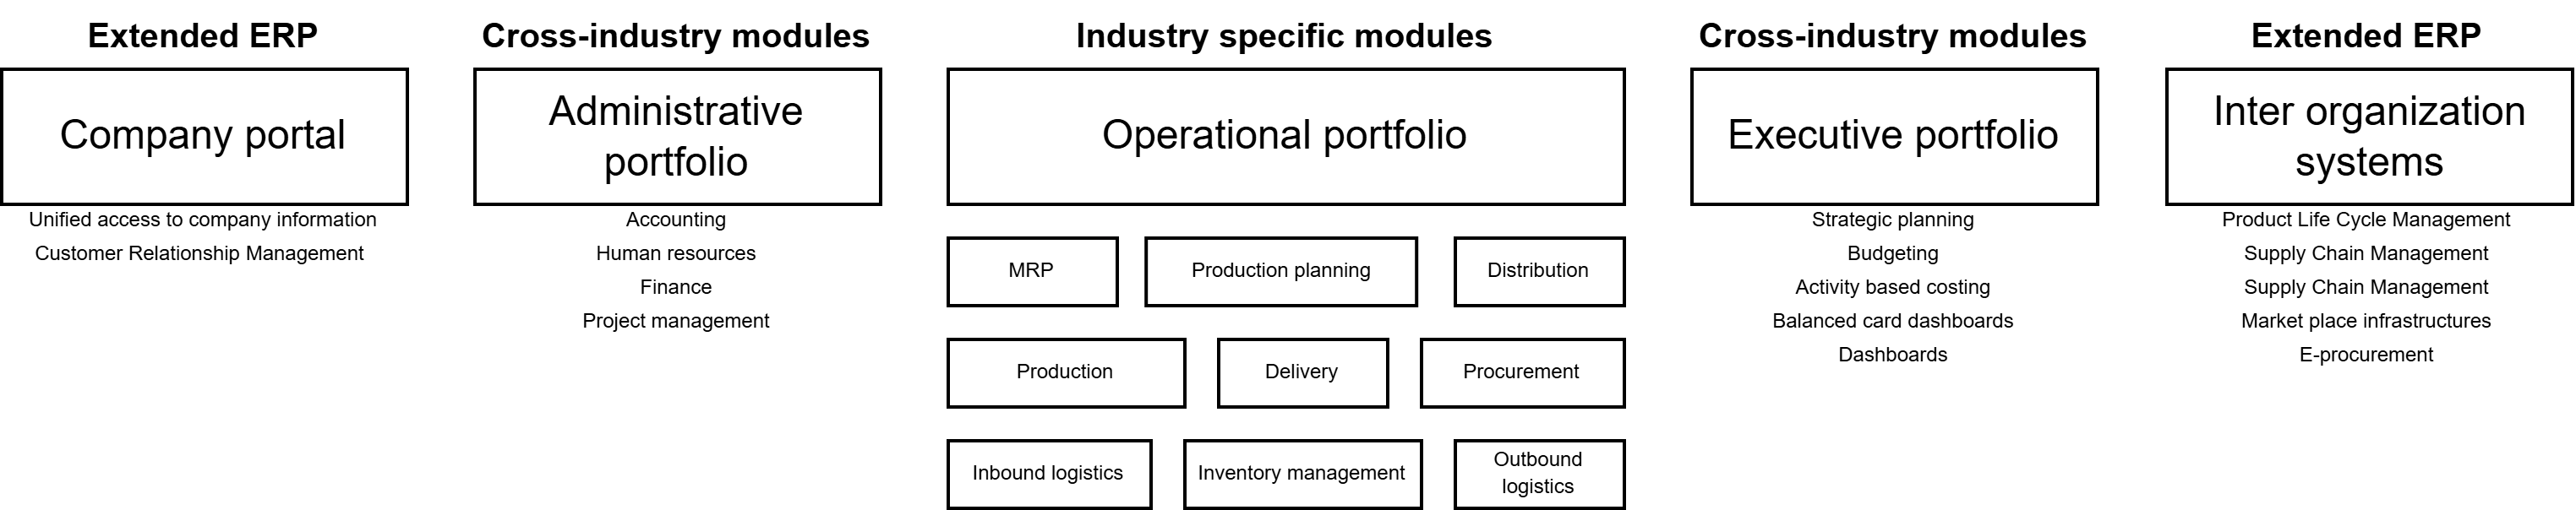
\includegraphics[width=1\linewidth]{images/bis1.png}
    \caption{ERP architecture}
\end{figure}
ERP stands for Enterprise Resource Planning. The acronym has been
coined in the mid ’90s by Gartner Group.
• There is an important distinction betweem:
– ERP modules supporting internal processes, called core ERP.
– ERP modules supporting the interaction with external parties, such as customers
and suppliers, called extended ERP.
Core ERP modules include: – Administrative portfolio
– Operational portfolio (industry dependent, vertical solutions)
– Executive portfolio
• Extended ERP modules include: – CRM, Customer Relationshiop Management,
– SCM, Supply Chain Management),
– E-Procurement and Market Place.

\subsection{Paradigm}
1) Information integration: ERP vision Decision-making applications, functionalities, user interfaces Operations support applications, functionalities, user interfaces Horizontal data consistency (information sharing)
• Vertical data consistency (from operations to executive dashboards)
• Conceptual consistency: one, common, integrated data model

2) Extension and modularity: Functional completeness
• Modularity:
– One Stop Shopping (one
supplier)
– Best of The Breed (multiple
suppliers)
3) Process prescriptiveness: ERP packages embed a process logic, e.g.: – “materials cannot be accepted without corresponding orders”
• Custom applications are develpoped ad hoc based on process requirements
• ERPs bring in a process and organizations have to change and conform to the logic
embedded in the ERP
• There are advantages (speed and costs) and disadvantages
(diversification/competitiveness)
Information integration: integrating legacy systems
ssues:
• Inconsistencies
• Slow batch alignment
• Obsolescence

• No single ERP provider can offer all functionalities for all industries
• There exist niche players focused on industry-specific functionalities (e.g. cashier
systems for the retail industry or machine-to-machine and machine-to-ERP integration
in manufacturing)
• There’s room for system integration to integrate sofware from different suppliers (or
with legacy systems)
• Small and medium size companies typically adopt:
– Simplified ERP packages (ERP light)
– Software as a service (SaaS) / Cloud-based solutions (e.g. Zoho, Magento, …)

ERP alternatives
• Large enterprise, revenues > 50
million euro
• Classic ERP
– BPR
– Industry-specific (vertical)
– System integration
– High costs
– Relatively long time frame (>6
months)
• SMEs
– Light ERPs “plug and play”
– No BPR
– Simple administrative
functionalities
– Simple analytics
– Limited scalability, need to change
ERP as company grows
ERPs complete integration
• We have talked about horizontal/vertical integration of portfolios
• ERPs complete integration of operational and executive with the administrative
portfolio
• This enables a real-time reconciliation of budgets, resource consumption, progress of
operations and cashflows
• Activity-based costing (ABC) represents a fundamental component of this integration

Activity based costing (ABC)
• Operations are associated with costs
• Operations can be associated with an internal pricing system
• Progress can be assessed from both a project management (time, quality) and financial
(cost) perspective
• Progress can be reconciled with administrative cash flows

Conclusions
So far, ERPs have integrated innovation into a unified solution.
Is this trend going to continue in the future?
Is cloud a threat to the ERP paradigm?
Is Gen AI a threat to the ERP paradigm?